\documentclass[11pt]{article}
\usepackage[utf8]{inputenc}
\usepackage{graphicx}
\usepackage[left=1.8cm, right=1.8cm, top=2cm, bottom=1.8cm]{geometry}
\usepackage{tabularx}
\usepackage{pbox}
\usepackage{physics}
\usepackage{booktabs}
\usepackage{fancyhdr}
\usepackage{enumitem}
\usepackage{multirow}
\usepackage{ctable}
\usepackage[medium]{titlesec}
\usepackage{wrapfig}
\titleformat*{\section}{\Large\bfseries}
\titleformat*{\subsection}{\large\bfseries}
\setlength{\textfloatsep}{2pt}
\pagestyle{fancy}


\title{Analyse Numérique : Devoir 3}
\author{Valentin Lemaire}
\date{9 décembre 2019}

\begin{document}
\rhead{Valentin Lemaire - 16341700}
\lhead{Devoir 3 : LU Creux}
\section{Format creux CSR}
\vspace{-10pt}
\subsection{Implémentation}
\vspace{-5pt}
La première version de la fonction (nommée \texttt{CSRformat\_slow} dans le code) parcourt les éléments de A et chaque fois qu'elle rencontre un élément non-nul, elle ajoute sa valeur à sA et son indice de colonne à jA, elle met également iA à jour a chaque ligne terminée. Cette fonction a été accélérée grâce à numpy dans \texttt{CSRformat}. Le nombre d'opérations exécutées par cette fonction (la version lente) est de approximativement $3N^2$ opérations où $N$ est le nombre d'inconnues du problème ($A$ est de dimension $N \cross N$). La fonction a un ordre $\mathcal{O}(N^2)$. \\
\vspace{-12pt}

\subsection{Evaluation des performances}
\begin{wrapfigure}[7]{r}{0.5\linewidth}
    \vspace{-50pt}
    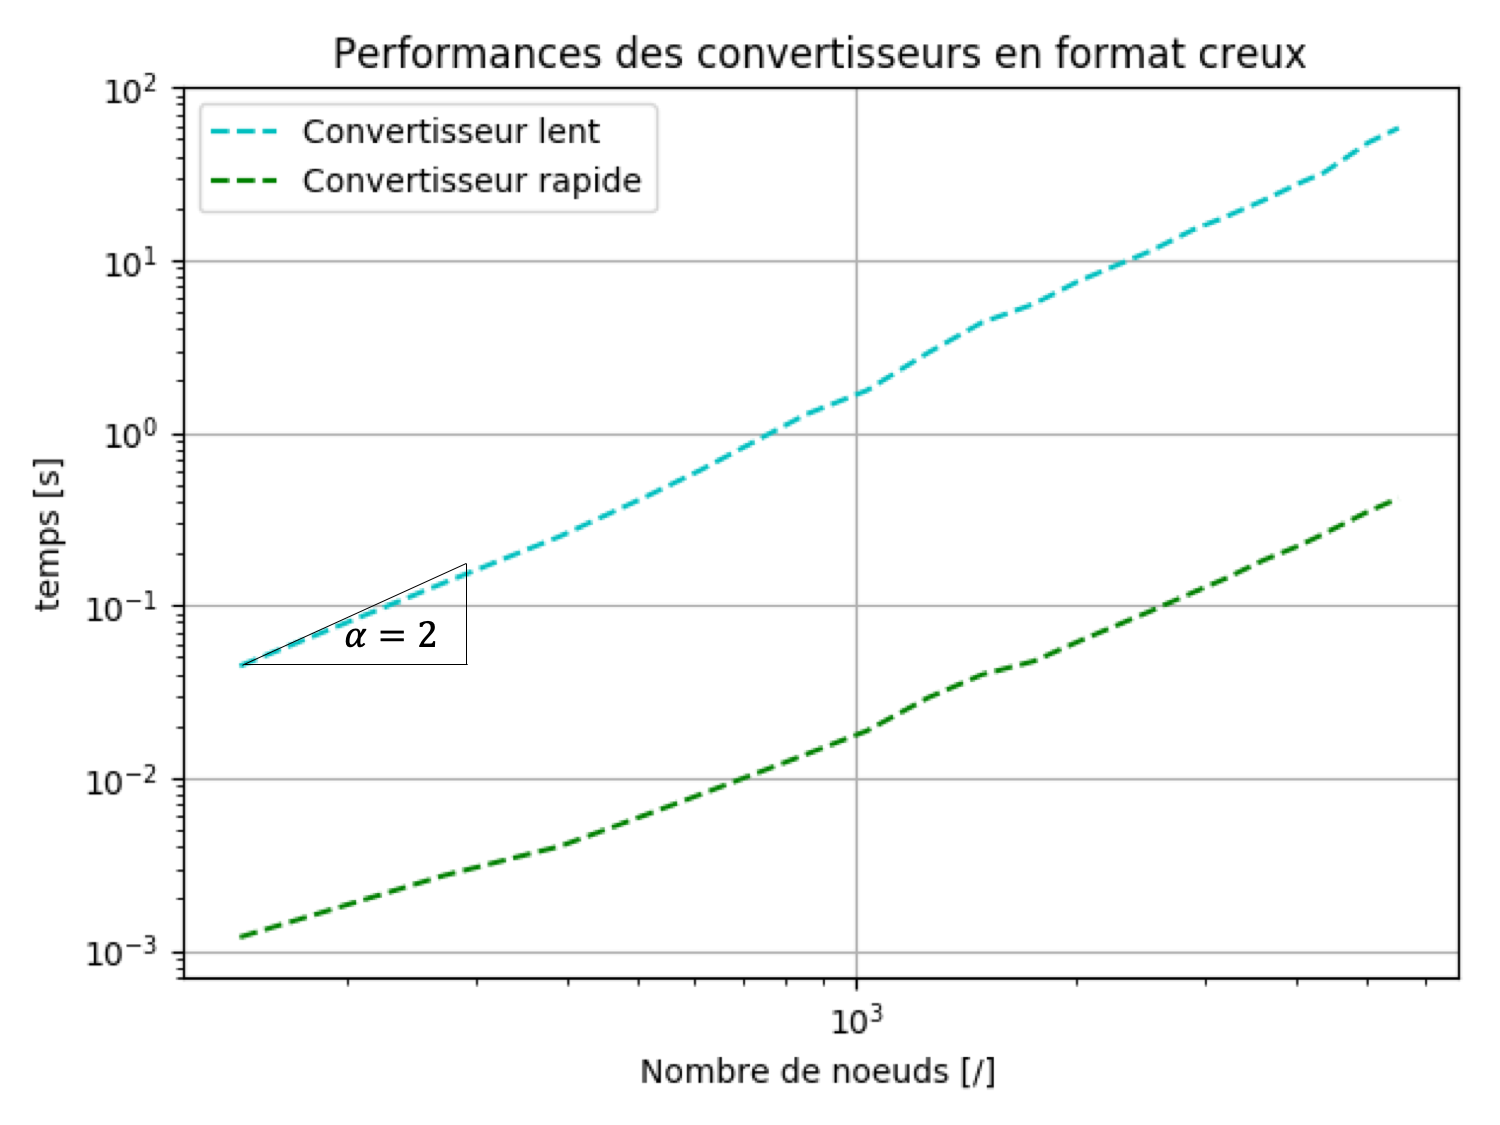
\includegraphics[width=0.45\textwidth]{csrformatperf.png}
    \vspace{-15pt}
    \caption{Performances des convertisseurs}
    \label{csrformatperf}
\end{wrapfigure}


Le graphe en figure \ref{csrformatperf}, montre que le temps pris pour transformer une matrice pleine en un format creux est effectivement proportionnel à $N^2$ (la pente est de 2 sur le graphe logarithmique). A titre informatif, le temps pris pour la version rapide a également été affiché sur le graphe. Elle est effectivement plus rapide (d'un facteur 100 approximativement). 


\section{LU creux}
\vspace{-8pt}
\subsection{Implémentation}
\vspace{-5pt}
La première version de l'implémentation de l'algorithme LU en format creux, nommée \texttt{LUcsr\_slow} commence par calculer les bandes à gauche et à droite de la diagonale (grâce à la fonction \texttt{compute\_bands\_slow}). Celle-ci va, pour chaque ligne calculer la différence entre l'indice du dernier élément non nul de la ligne (resp. l'indice de la ligne) et l'indice  de la ligne (resp. du premier élément non-nul de la ligne) pour calculer les bandes supérieures et inférieures à cette ligne et va renvoyer les maximums sur toutes les lignes de ces deux valeurs. Le nombre d'opérations pour cette fonction est approximativement $4N$ et son ordre est donc $\mathcal{O}(N)$\footnote{Pour toutes les valeurs de nombre d'opérations dans ce rapport, un calcul détaillé se trouve en Annexe}.\\
\vspace{-8pt}

Ensuite, vient la création du "pseudo format creux" dans \texttt{create\_fill\_in} qui est, comme le vrai format creux, un trio de vecteurs (ici baptisés sLU, iLU et jLU) qui contiennent les mêmes valeurs que sA, iA et jA mais en plus de ces valeurs, il y aura des 0 dans sLU et les indices correspondants dans iLU et jLU partout où la décomposition LU va potentiellement générer du fill-in. Cela permet de pré-allouer toutes les entrées que LU va potentiellement modifier et donc faciliter l'implémentation de la décomposition. Cette fonction a un nombre d'opérations valant approximativement $4NB$ (où $B$ est la largeur de la bande, définie comme le maximum entre la bande supérieure et la bande inférieure) et l'odre de la fonction est donc $\mathcal{O}(NB)$\\ 
\vspace{-8pt}

Après cela, la fonction procède à la décomposition LU à proprement dite. Cela est fait en tirant profit du "pseudo format creux" défini ci-dessus et du fait que la décomposition LU ne modifie que les éléments dans la bande. Ainsi, à l'itération $i$, seuls les $b_l$ éléments de la colonne $i$ qui sont dans la bande (où $b_l$ est la bande inférieure) seront divisés et pas tous les éléments allant de $i$ à $N-1$. De la même manière, au lieu de faire $a_{jk} = a_{jk} - a_{ji}a_{ik}$ pour tout $j$ et pour tout $k$ allant de $i+1$ à $N-1$, ce n'est fait que pour $j$ allant de $i+1$ à $min(i+1+b_l, N-1)$ et $k$ allant de $i+1$ à $min(i+1+b_u, N-1)$ puisque faire le calcul pour les autres éléments ne modifiera pas les valeurs dans sLU (le produit $a_{ji}a_{ik}$ est nul pour l
ces valeurs de $j$ et $k$). Cette implémentation a un nombre d'opérations valant approximativement $3NB^2 - 2B^3$ et donc un ordre $\mathcal{O}(NB^2)$ car $N \ge B$\\
\vspace{-8pt}

Enfin, la fonction \texttt{remove\_zeros\_slow} va parcourir le vecteur sLU obtenu après la décomposition LU et enregistrer dans un nouveau vecteur tous les éléments non-nuls pour ré-obtenir un véritable format creux. Cette fonction a un nombre d'opérations valant approximativement $6NB$ et son ordre est donc $\mathcal{O}(NB)$. C'est le résultat de cette fonction qui sera renvoyé lorsqu'on appelle la fonction \texttt{LUcsr\_slow}.
\vspace{-8pt}

\paragraph{Remarque} toutes les fonctions qui se terminenet par "\texttt{\_slow}" ont un équivalent qui utilise des fonctions numpy et qui sont plus rapides mais ce ne sont pas celles utilisées pour étudier les complexités. Les détails de ces calculs de complexités se trouvent en Annexe.
\vspace{-8pt}


\section{Reverse Cuthill McKee}
\begin{wrapfigure}[15]{r}{0.6\textwidth}
    \centering
    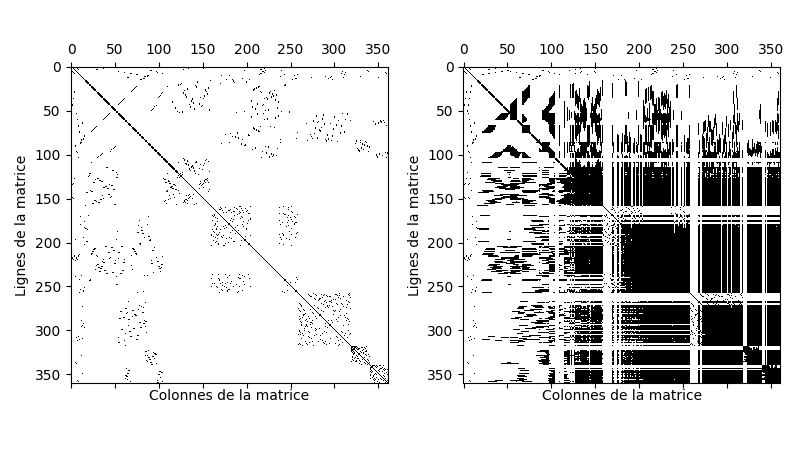
\includegraphics[width=\linewidth]{mask_matrices_no_rcmk.png}
    \vspace{-1.5cm}
    \caption{Masque des matrices A et LU avant et après l'application de l'algorithme LU}
    \label{masksbeforercmk}

\end{wrapfigure}
\vspace{-10pt}

L'algorithme LU ne crée pas de fill-in hors de la bande. Il est donc très intéressant de travailler avec des matrices qui sont bandes pour résoudre des systèmes linéaires creux. Cependant, pour une matrice d'éléments finis, il n'y a pas de raison qu'elle soit bande au départ. Et en effet, la figure \ref{masksbeforercmk} montre le masque de la matrice $A$ (obtenue avec $f=50Hz$ et $vel = 0$ et 393 noeuds) avant l'application de l'algorithme LU et celui de la matrice retournée après l'application de l'algorithme LU (symbolique des matrices $L$ et $U$). Ici, comme la largeur de la bande est très grande (les éléments sont répartis dans presque toute la matrice et donc la largeur de bande $B$ est comparable aux nombres d'inconnues du système $N$, on a $B \approx N$) le fill-in se fait sur presque l'entièreté de la matrice. \\
\vspace{-8pt}


\begin{wrapfigure}[16]{r}{0.6\textwidth}
    \centering
    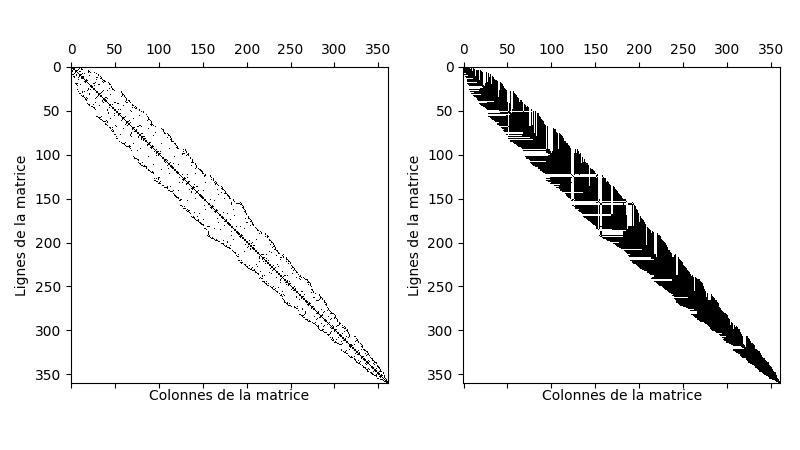
\includegraphics[width=\linewidth]{mask_matrices_with_rcmk.png}
    \vspace{-1.5cm}
    \caption{Masque des matrices A et LU avant et après l'application de l'algorithme LU en utilisant la permutation de RCMK}
    \label{masksafterrcmk}

\end{wrapfigure}

L'algorithme RCMK est une heuristique qui permet de réduire considérablement la bande d'une matrice creuse. Elle ne trouve cependant pas la bande optimale (c'est un problème NP-complet\footnote{Billionnet A., Brêteau J.-F., 'A comparison of three algorithms for reducing the profile of a sparse matrix', \textit{
Revue française d’automatique, d’informatique et de recherche opérationnelle}. Recherche opérationnelle, tome 23, no 3 (1989), p. 289-302.}). \\
\vspace{-8pt}

La figure \ref{masksafterrcmk} représente l'état du masque de la matrice de départ $A$ à laquelle on a appliqué le vecteur de permutation obtenu par RCMK comme il est défini dans le cours ainsi que le fill-in de cette matrice suite à l'application de l'algorithme LU. La figure montre que la bande est fortement réduite et que le fill-in est nettement moins important si on applique la permutation.\\
\vspace{-8pt}

Le tableau \ref{tablercmk} fournit des valeurs pour les tailles de bandes pour différents maillages avant et après l'application du vecteur de permutation obtenu par RCMK. Il contient également le pourcentage initial d'éléments non-nuls dans la matrice $A$ et le pourcentage d'éléments non-nuls dans la matrice LU (représentatif de la quantité d'éléments non-nuls des matrices $L$ et $U$) et ce, dans le cas où le cas où la permutation par RCMK a été appliquée et dans le cas où ce n'est pas fait. Les résultats montrent que la bande est fortement réduite et que le fill-in est beaucoup moins important si RCMK est appliqué.\\ 
% \vspace{-8pt}

\begin{table}[]
    \centering
    \begin{tabular}{|c|c|c|c|c|}
        \hline
         & 143 noeuds & 393 noeuds & 610 noeuds & 1033 noeuds\\
        \hline
         Taille de la bande avant RCMK & 116 & 351 & 552 & 957 \\
        \hline
         Taille de la bande après RCMK & 26 & 38 & 40 & 80 \\
        \hline
         Eléments non-nuls avant LU [\%] & 5.08 & 1.85 & 1.20 &  0.705 \\
        \hline
         Eléments non-nuls après LU sans RCMK [\%] & 45.06 & 49.47 & 38.89 &  26.08 \\
        \hline
         Eléments non-nuls après LU avec RCMK [\%] & 24.21 & 10.74 & 8.56 & 8.61 \\
        \hline
    \end{tabular}
    \caption{Bande et sparisté de la matrice avec RCMK}
    \label{tablercmk}
\end{table}
\vspace{-8pt}

\subsection{Implémentation}
L'alorithme Reverse Cuthill McKee a été implémenté dans la fonction \texttt{RCMK} de la manière suivante. La fonction initialise le vecteur r et la queue q (implémenté sous forme de liste de taille N car on n'ajoutera jamais plus d'éléments à la queue que le nombre total de noeuds). Elle applique ensuite l'algorithme RCMK en ajoutant dans r soit le noeud de degré minimum (n'ayant pas déjà été mis dans r) si q est vide, soit le premier élément de q dans l'ordre inverse (en partant de r[N-1] et en descendant dans les indices) et ajoute dans q les voisins du noeud qui a été ajouté à r (qui n'ont pas déjà été ajoutés à q ou r) grâce à deux indices \texttt{q\_i} et \texttt{q\_j} où \texttt{q[q\_i]} est le premier élément dans la queue et \texttt{q\_j} est l'indice juste après le dernier élément de q. Les voisins sont triés par ordre croissant de degré grâce à la fonction \texttt{sorted}. RCMK a un nombre d'opérations proportionnel à $(C+1)N$ où $C$ est une constante positive définie dans le calcul de complexité pour RCMK en Annexe. L'ordre de la fonction est donc $\mathcal{O}(N)$.\\
\vspace{-8pt}

L'application de la permutation au format creux a été implémentée de la manière suivante. On itère sur $N$, et à chaque itération $i$ on ajoute dans un nouveau de trio de vecteurs les éléments correspondants à la ligne \texttt{r[i]}. Cette ligne est ensuite réarrangée pour que les indices des colonnes se trouvent par ordre croissant dans jLU (sLU est donc également modifié). Cette fonction a un nombre d'opérations de approximativement $CN$ et son ordre est donc $\mathcal{O}(N)$. Une fois de plus les détails du calcul se trouvent en Annexe.
\vspace{-8pt}

\section{Résolution du système creux}
\vspace{-10pt}
La fonction \texttt{LUsolve\_csr\_slow} résout les deux systèmes triangulaires $Ly = b$ et $Ux = y$. Elle parcourt ainsi deux fois le trio de vecteurs sLU, iLU et jLU en faisant des opérations matricielles avec les vecteur \texttt{b}, \texttt{y} et \texttt{x} pour trouver la solution. Cette fonction a un nombre d'opérations de approximativement $4NQ$ où $Q$ est une constante positive définie en Annexe avec le détail du calcul. L'ordre de la fonction est $\mathcal{O}(N)$.
\vspace{-8pt}

\section{Complexité de la résolution du système $Ax = b$}
\vspace{-10pt}
La complexité pour résoudre le système linéaire $Ax = b$ dans le cas du régime dynamique du problème est donnée ci-dessous.
\vspace{-8pt}

\paragraph{Sans RCMK} Il faut sommer les nombres d'opérations pour le convertisseur, la décomposition LU et le solveur, cela donne : $N_{op} \approx 3N^2 + 2N + 4NB + 3NB^2 - 2B^3 + 6NB + 4NQ \approx  3NB^2 - 2B^3$. Comme quand on applique pas RCMK, $B \approx N$. Cela donne : $N_{op} \approx N^3$. L'ordre est donc $\mathcal{O}(N^3)$
\vspace{-8pt}

\paragraph{Avec RCMK} Il faut cette fois ajouter au résultat précédent les nombres d'opérations pour obtenir le vecteur de permutation et pour l'appliquer, cela donne : $N_{op} \approx 3N^2 + 2N + 4NB + 3NB^2 - 2B^3 + 6NB + (C+1)N + CN + 4NQ \approx   3NB^2 - 2B^3$. \\Lorsque RCMK est appliqué, $B << N$, donc $2B^3 << 2NB^2$ et donc $N_{op} \approx 3NB^2$. L'ordre est $\mathcal{O}(NB^2)$\\
\vspace{-8pt}

En observant le graphe en figure \ref{perf-graph}, où sont représentés les temps d'exécutions des différents algorithmes, il est évident que sur une matrice d'éléments finis, exécuter l'algorithme LU creux avec RCMK est plus rapide (cela vient du fait que la vitesse de LU dépend de la largeur $B$ de la bande). \\
\vspace{-8pt}

Ce même graphe montre également que l'algorithme LU plein et LU creux sans RCMK sont tous les deux en $\mathcal{O}(N^3)$ et diffèrent d'une constante (LU plein est plus rapide d'un facteur 3/2 en l'occurence, ce qui colle avec les valeurs théoriques). \\

\begin{figure}
    \begin{minipage}{0.5\linewidth}
    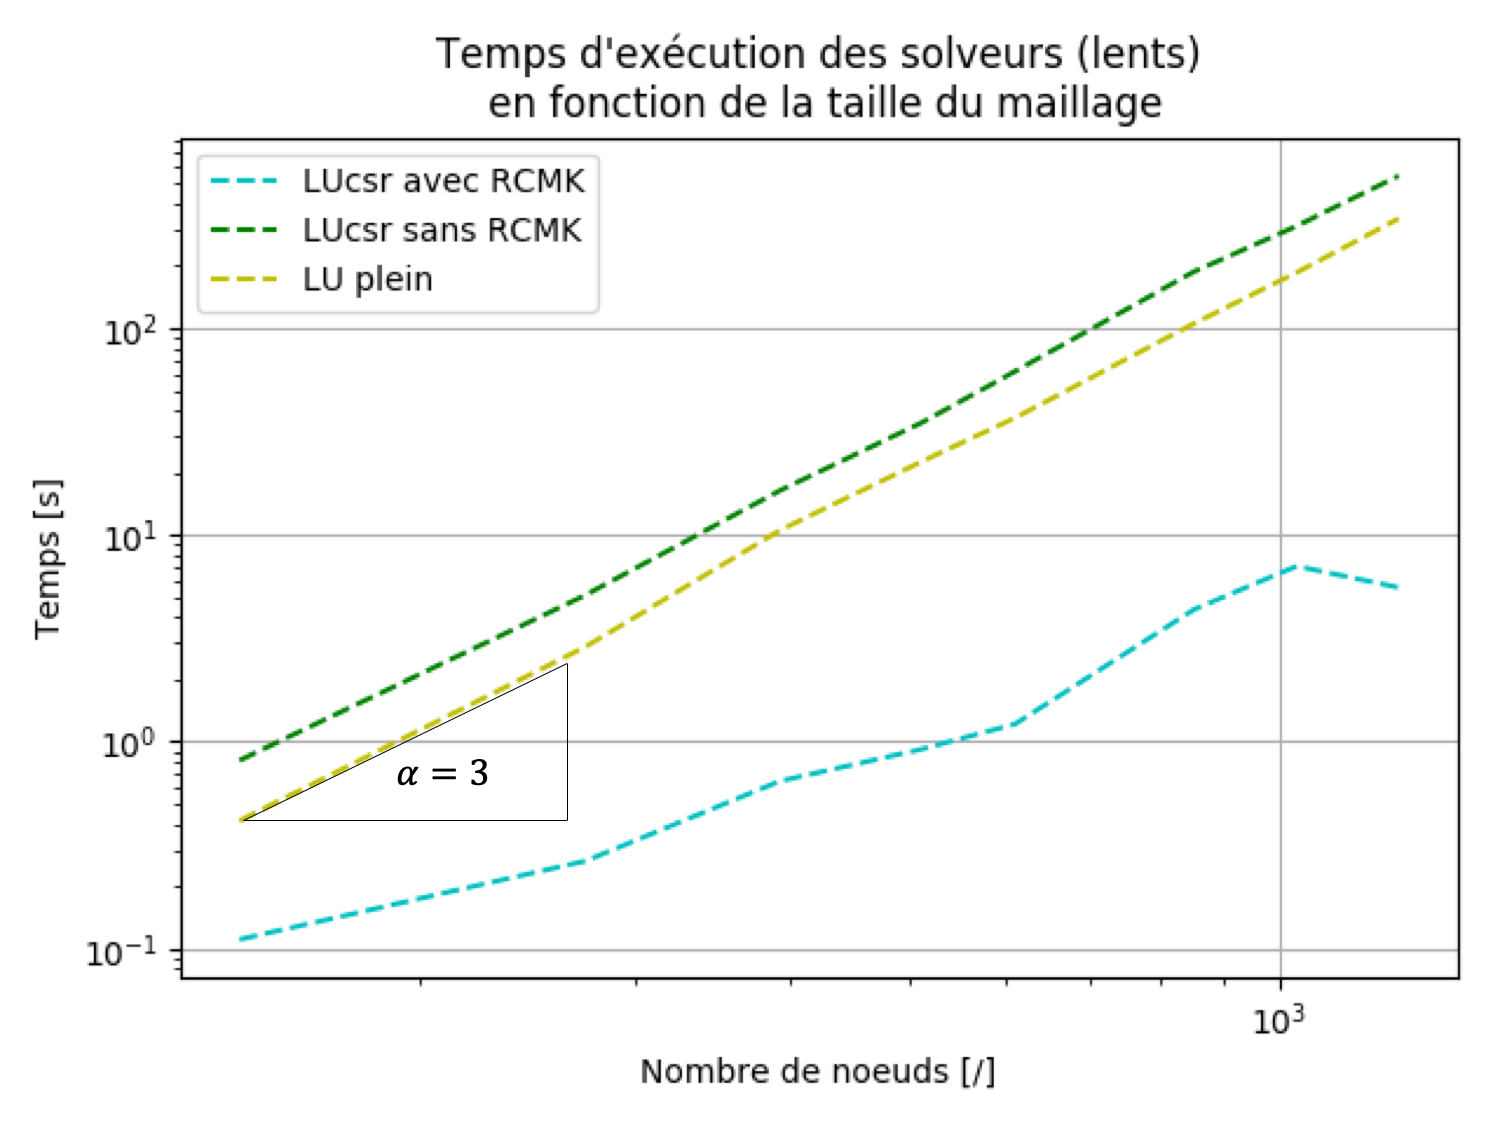
\includegraphics[width = \textwidth]{graph_slow.png}
    \end{minipage}\hfill 
    \begin{minipage}{0.5 \linewidth}
    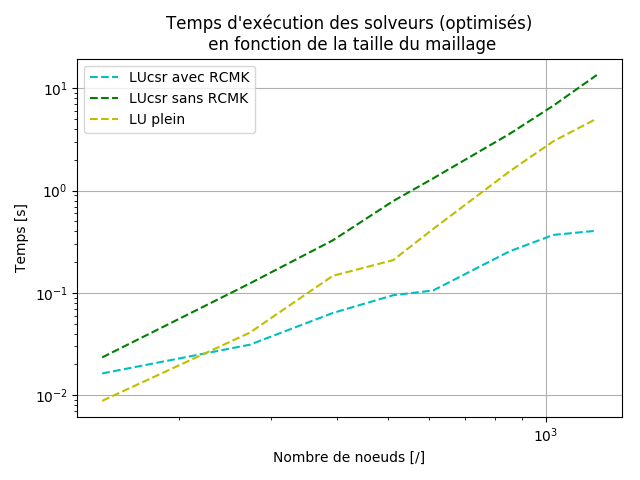
\includegraphics[width = \textwidth]{graph_opt.png}
    \end{minipage}
    \caption{Performances des différentes méthodes de résolution du système linéaire}
    \label{perf-graph}
\end{figure}

La résolution avec matrices creuses et en utilisant RCMK est beaucoup plus rapide que sans RCMK ou la résolution en matrice pleine. Et résoudre une matrice qui n'est pas bande avec le format creux est plus lent que de la résoudre avec le format plein\footnote{Pour pouvoir faire la meilleure comparaison, la décomposition LU pleine a été faite sans pivotage}.\\
\vspace{-8pt}

En effet, lorsque RCMK n'est pas appliqué, la valeur de $B$ sera égale (ou presque) à $N$ (on n'a pas réduit la bande), le nombre d'opérations est alors : $N_{op} \approx 3N^3 - 2N^3 = N^3$ (ce qui est sensiblement plus que les $2\frac{N^3}{3}$ du format LU plein). Cependant, appliquer RCMK réduit considérablement la bande, donc $B << N$ et $N_{op} \approx 3NB^2 - 2B^3 \approx 3NB^2 << 2\frac{N^3}{3}$. Ce qui explique la performance largement supérieure de LU creux avec RCMK. \\
\vspace{-8pt}

Le temps d'exécution de la décomposition LU creuse avec RCMK est nettement plus avantageux. Et comme le montre le tableau \ref{precisionsolveurs}, cela ne se fait pas au détriment de la précision. En effet, c'est également une méthode directe et sa précision est comparable à celles des autres solveurs et surtout à celui de numpy, utilisé comme référence (c'est une comparaison des différents solveurs avec $f = 50Hz$, $vel = 0$ et 1033 noeuds).
\begin{table}[]
    \centering
    \begin{tabular}{|c|c|c|c|c|}
        \hline
         &  numpy & LU plein & LU creux sans RCMK & LU creux avec RCMK\\
         \hline
         $||Ax - b||_2/||b||_2$ [/] & $2.26 \cdot 10^{-14}$ &  $4.05 \cdot 10^{-14}$ & $4.04 \cdot 10^{-14}$ & $3.39\cdot 10^{-14}$\\
         \hline
    \end{tabular}
    \caption{Précisions des différents solveurs}
    \label{precisionsolveurs}
\end{table}
\vspace{-12pt}

\section{Permuter avec un format creux}
\vspace{-10pt}
Avec un format creux, ce serait une mauvaise idée d'appliquer les permutations pour éviter de tomber sur un pivot non-nul, en effet, l'intérêt de travailler en creux est de réduire la bande par RCMK. Et si la matrice est bande, permuter une ligne $i$ avec une ligne $j$ va potentiellement engendrer des valeurs non-nulles hors de l'espace pré-alloué (la ligne $i$ peut avoir des éléments allant de $i - b_l$ à $i + b_u$) mais rien ne garantit que les éléments non-nuls de la ligne $j$ seront compris entre ces indices. De plus, même si les éléments correspondants étaient ajoutés, la bande $B$ serait potentiellement modifiée et le fill-in serait plus important (ce qui ralentirait les performances de l'algorithme). Enfin, ceci n'aurait pas de réelle utilité dans une matrice d'éléments finis où la diagonale est toujours non-nulle. 

\section*{Annexe}
\vspace{-10pt}
\subsection*{Nombre d'opérations du convertisseur}
Le code (en version avec des boucles for) parcourt la matrice et pour chaque élément non-nul incrémente le compteur et ajoute un élément à sA et un autre à jA via la fonction append (qui en moyenne, prend un temps en $\theta(1)$ d'après la documentation python). : 
\begin{equation}
    N_{op} = \sum_{i=0}^{N-1} \left(1 + \sum_{j = 0}^{N-1} 3\right) + (petit) = 3N^2 + (petit) \approx 3N^2
\end{equation}
\vspace{-15pt}

\subsection*{Nombre d'opérations de la décomposition LU creuse}
En ne comptant que les opérations de calcul (addition, multiplication, etc.), les nombres d'opérations pour les fonctions relatives à la décomposition sont les suivants
\vspace{-8pt}
\paragraph{Calcul des bandes} (\texttt{compute\_bands\_slow}) 
\begin{equation}
    N_{op} = \sum_{i=0}^{N-1} 4 + (petit) \approx 4N
\end{equation}\label{eq1}
\vspace{-15pt}
\paragraph{Création du pseudo format CSR} (\texttt{create\_fill\_in}), dans le pire des cas, on ne rajoute pas de 0 au format creux et pour chaque ligne, on rajoute 2B+1 éléments de sA dans sLU 
\begin{equation}
    N_{op} = \sum_{i=0}^{N-1} \left(1 + \sum_{j=0}^{2B} 1 + 1 + \sum_{j=0}^{2B} 1\right) = N(2B+1) + N(2B+1) + (petit) \approx 4NB
\end{equation}\label{eq2}
\vspace{-15pt}
\paragraph{Algorithme LU creux} Ici, $b_i$ vaut : $b_i = B - (N - 1) + i$ si ce nombre est positif et 0 sinon. On a 3 opérations dans la 3ème somme car on fait les opérations de multiplication et de soustraction pour LU mais on doit également faire une somme dans l'appel des indices. 
\begin{equation}
    N_{op} = \sum_{i=0}^{N-1}\left(\sum_{j=i+1}^{i + B - b_i} \left( 1 + \sum_{k=i+1}^{i + B - b_i} 3\right)\right) + (petit) = 3(N-B)B B + 6\frac{B^3}{3}+ (petit) \approx 3NB^2 -  2B^3
\end{equation}\label{eq3}
\vspace{-15pt}
\paragraph{Retrait des zeros restants} (\texttt{remove\_zeros\_slow}) Ici, $s_i$ représente l'indice du premier élément de la ligne i dans sLU
\begin{equation}
    N_{op} = \sum_{i=0}^{N-1}\left( 1 + \sum_{j = s_i}^{s_i + 2B} 3\right) + (petit) = N(1 + 3(2B+1)) + (petit) \approx 6NB
\end{equation}\label{eq4}
\vspace{-15pt}

\subsection*{Nombre d'opérations et ordre pour RCMK}
\paragraph{Calcul du vecteur de permutation} Dans le cadre d'une matrice d'éléments finis, en faisant l'analogie avec une matrice d'adjacence, le graphe est toujours connexe (il n'y a pas de séparations dans le maillage). L'algorithme va, pour chaque composante connexe (ici il n'y en a qu'une), rechercher le noeud de degré minimum et ensuite les itérer sur les noeuds voisins à celui-là et puis sur leurs voisins, etc. Pour chaque noeud qu'il met dans r, il doit récupérer les voisins, les trier selon leur degrés et les placer dans q. La fonction utilisée pour trier a un ordre $O(nlog(n))$ où n est la taille de la liste a trier, comme chaque noeud a un nombre de voisins borné par une constante (peu importe la taille du maillage), le tri et les autres opérations de la boucle se font en temps constant. En nommant cette constante $C$, le nombre d'opérations devient.
\begin{equation}
    N_{op} = \sum_{i = 0}^{N-1} 1 + \sum_{i = 1}^{N-1} C + (petit) \approx (C+1)N
\end{equation}
\vspace{-15pt}

\paragraph{Application de la permutation} A chaque itération, il faut placer et trier les voisins d'un noeud, le nombre d'opérations par itération est donc proche de $C$
\begin{equation}
    N_{op} \approx \sum_{i = 0}^{N-1} C + (petit) \approx C N
\end{equation}
\vspace{-20pt}

\subsection*{Nombre d'opérations du solveur}
Soit $V_i$ l'ensemble des noeuds voisins au noeud i, le nombre d'opérations de cette fonction peut s'écrire comme suit
\begin{equation}
    N_{op} = \sum_{i = 0}^{N-1}\left( \sum_{j \in V_i} 2 \right) + \sum_{i = 0}^{N-1}\left( 1 + \sum_{j \in V_i} 2 \right) + (petit)
\end{equation}
Comme le nombre de voisins du noeud $i$ est borné à 9, $|V_i| \leq 9$, $\sum_{j \in V_i} 1 \leq constante = Q$, on a :
\begin{equation}
    N_{op} = \sum_{i = 0}^{N-1}2Q + \sum_{i = 0}^{N-1}2Q + (petit) \approx 4NQ
\end{equation}
\end{document}